% algorithmes de plus courts chemins 

\begin{frame}{Graphes pondérés}

\begin{definition}
    Un graphe \emph{non-orienté pondéré} est un graphe non-orienté muni d'une fonction de pondération qui associe une valeur réelle à chaque arête. 
\end{definition}

\begin{definition}
    Un graphe \emph{orienté pondéré} est un graphe orienté muni d'une fonction de pondération qui associe une valeur réelle à chaque arc. 
\end{definition}

\end{frame}

\begin{frame}{Exemple : graphe non-orienté pondéré}
    \begin{center}
        \begin{tikzpicture}
\clip (0,0) rectangle (6,6);
\Vertex[x=0.450,y=5.550,size=0.8,opacity=0.5,label=1]{0}
\Vertex[x=0.450,y=3.000,size=0.8,opacity=0.5,label=2]{1}
\Vertex[x=3.000,y=3.000,size=0.8,opacity=0.5,label=3]{2}
\Vertex[x=3.000,y=5.550,size=0.8,opacity=0.5,label=4]{3}
\Vertex[x=5.550,y=5.550,size=0.8,opacity=0.5,label=5]{4}
\Vertex[x=5.550,y=3.000,size=0.8,opacity=0.5,label=6]{5}
\Vertex[x=5.550,y=0.450,size=0.8,opacity=0.5,label=7]{6}
\Vertex[x=3.000,y=0.450,size=0.8,opacity=0.5,label=8]{7}
\Vertex[x=0.450,y=0.450,size=0.8,opacity=0.5,label=9]{8}
\Edge[,lw=2.0,bend=-8.531,label=5](0)(1)
\Edge[,lw=2.0,bend=-8.531,label=2](0)(3)
\Edge[,lw=2.0,bend=-8.531,label=-2](1)(3)
\Edge[,lw=2.0,bend=-8.531,label=4](2)(8)
\Edge[,lw=2.0,bend=-8.531,label=1](4)(5)
\Edge[,lw=2.0,bend=-8.531,label=3](5)(6)
\Edge[,lw=2.0,bend=-8.531,label=0](6)(7)
\end{tikzpicture}

    \end{center}
    \end{frame}

% TODO exemple de graphe orienté avec pondération ?

\begin{frame}{Applications}
    \begin{itemize}
        \item Calcul de plus courts chemins 
        \begin{itemize}
            \item Distances entre villes
        \end{itemize}
        \item Arbres couvrants minimaux 
        \item Contraintes entre tâches 
    \end{itemize}
\end{frame}

\begin{frame}{Arbre couvrant}
    \begin{definition}
        Dans un graphe $G$ non orienté (pondéré ou non) connexe, un arbre couvrant est un sous-graphe connexe acyclique (arbre) incluant tous les sommets de $G$
    \end{definition}


\end{frame}

% TODO ajouter définition d'un sous-graphe 


\begin{frame}{Exemple : arbre couvrant}
    \begin{center}
        \begin{tikzpicture}
\clip (0,0) rectangle (6,6);
\Vertex[x=0.450,y=5.550,size=0.8,opacity=0.5,label=1]{0}
\Vertex[x=0.450,y=3.000,size=0.8,opacity=0.5,label=2]{1}
\Vertex[x=3.000,y=3.000,size=0.8,opacity=0.5,label=3]{2}
\Vertex[x=3.000,y=5.550,size=0.8,opacity=0.5,label=4]{3}
\Vertex[x=5.550,y=5.550,size=0.8,opacity=0.5,label=5]{4}
\Vertex[x=5.550,y=3.000,size=0.8,opacity=0.5,label=6]{5}
\Vertex[x=5.550,y=0.450,size=0.8,opacity=0.5,label=7]{6}
\Vertex[x=3.000,y=0.450,size=0.8,opacity=0.5,label=8]{7}
\Vertex[x=0.450,y=0.450,size=0.8,opacity=0.5,label=9]{8}
\Edge[,lw=2.0,bend=-8.531](0)(1)
\Edge[,lw=4.0,bend=-8.531](0)(3)
\Edge[,lw=4.0,bend=-8.531,](1)(3)
\Edge[,lw=4.0,bend=-8.531](2)(8)
\Edge[,lw=4.0,bend=-8.531](4)(5)
\Edge[,lw=4.0,bend=-8.531](5)(6)
\Edge[,lw=4.0,bend=-8.531](6)(7)
\Edge[,lw=4.0,bend=-8.531](3)(4)
\Edge[,lw=4.0,bend=-8.531](2)(6)
\Edge[,lw=2.0,bend=-8.531](2)(1)
\end{tikzpicture}

    \end{center}
    \end{frame}

    \begin{frame}{Contre-exemple : arbre non couvrant}
        \begin{center}
            \begin{tikzpicture}
\clip (0,0) rectangle (6,6);
\Vertex[x=0.450,y=5.550,size=0.8,opacity=0.5,label=1]{0}
\Vertex[x=0.450,y=3.000,size=0.8,opacity=0.5,label=2]{1}
\Vertex[x=3.000,y=3.000,size=0.8,opacity=0.5,label=3]{2}
\Vertex[x=3.000,y=5.550,size=0.8,opacity=0.5,label=4]{3}
\Vertex[x=5.550,y=5.550,size=0.8,opacity=0.5,label=5]{4}
\Vertex[x=5.550,y=3.000,size=0.8,opacity=0.5,label=6]{5}
\Vertex[x=5.550,y=0.450,size=0.8,opacity=0.5,label=7]{6}
\Vertex[x=3.000,y=0.450,size=0.8,opacity=0.5,label=8]{7}
\Vertex[x=0.450,y=0.450,size=0.8,opacity=0.5,label=9]{8}
\Edge[,lw=2.0,bend=-8.531](0)(1)
\Edge[,lw=4.0,bend=-8.531](0)(3)
\Edge[,lw=4.0,bend=-8.531,](1)(3)
\Edge[,lw=4.0,bend=-8.531](2)(8)
\Edge[,lw=2.0,bend=-8.531](4)(5)
\Edge[,lw=4.0,bend=-8.531](5)(6)
\Edge[,lw=4.0,bend=-8.531](6)(7)
\Edge[,lw=4.0,bend=-8.531](3)(4)
\Edge[,lw=4.0,bend=-8.531](2)(6)
\Edge[,lw=2.0,bend=-8.531](2)(1)
\end{tikzpicture}

        \end{center}
        \end{frame}
    
\begin{frame}{Construction d'un arbre couvrant}
\begin{itemize}
    \item Connaissez-vous un algorithme capable de construire un arbre couvrant ?
    \pause \item Oui !
    \pause \item Tous les algorithmes de parcours que nous avons vus jusqu'ici 
    \pause \item Pour de bonnes raisons applicatives, on va chercher à construire un arbre couvrant \emph{minimal} 
    \pause \item Est-on obligés de parcourir l'ensemble des arbres couvrants pour trouver un arbre de coût minimal ?
\end{itemize}
    
\end{frame}

\begin{frame}{Applications}
    \begin{itemize}
        \item Minimiser la longueur de câble nécessaire pour connecter un réseau 
        \item Heuristique dans certains problèmes d'optimisation
        \begin{itemize}
            \item problème du voyageur de commerce
        \end{itemize}
    \end{itemize}
\end{frame}

\begin{frame}{Arbre couvrant minimal}
    \begin{definition}
        Dans un graphe non orienté pondéré et connexe, un arbre couvrant minimal est un arbre couvrant dont la somme des arêtes est minimale
    \end{definition}

    \begin{itemize}
        \item Remarque : si le graphe n'est pas pondéré, on considère des arêtes de poids identique 
    \end{itemize}
\end{frame}

\begin{frame}{Exemple 1 : arbre couvrant minimal (non pondéré)}
    \begin{center}
        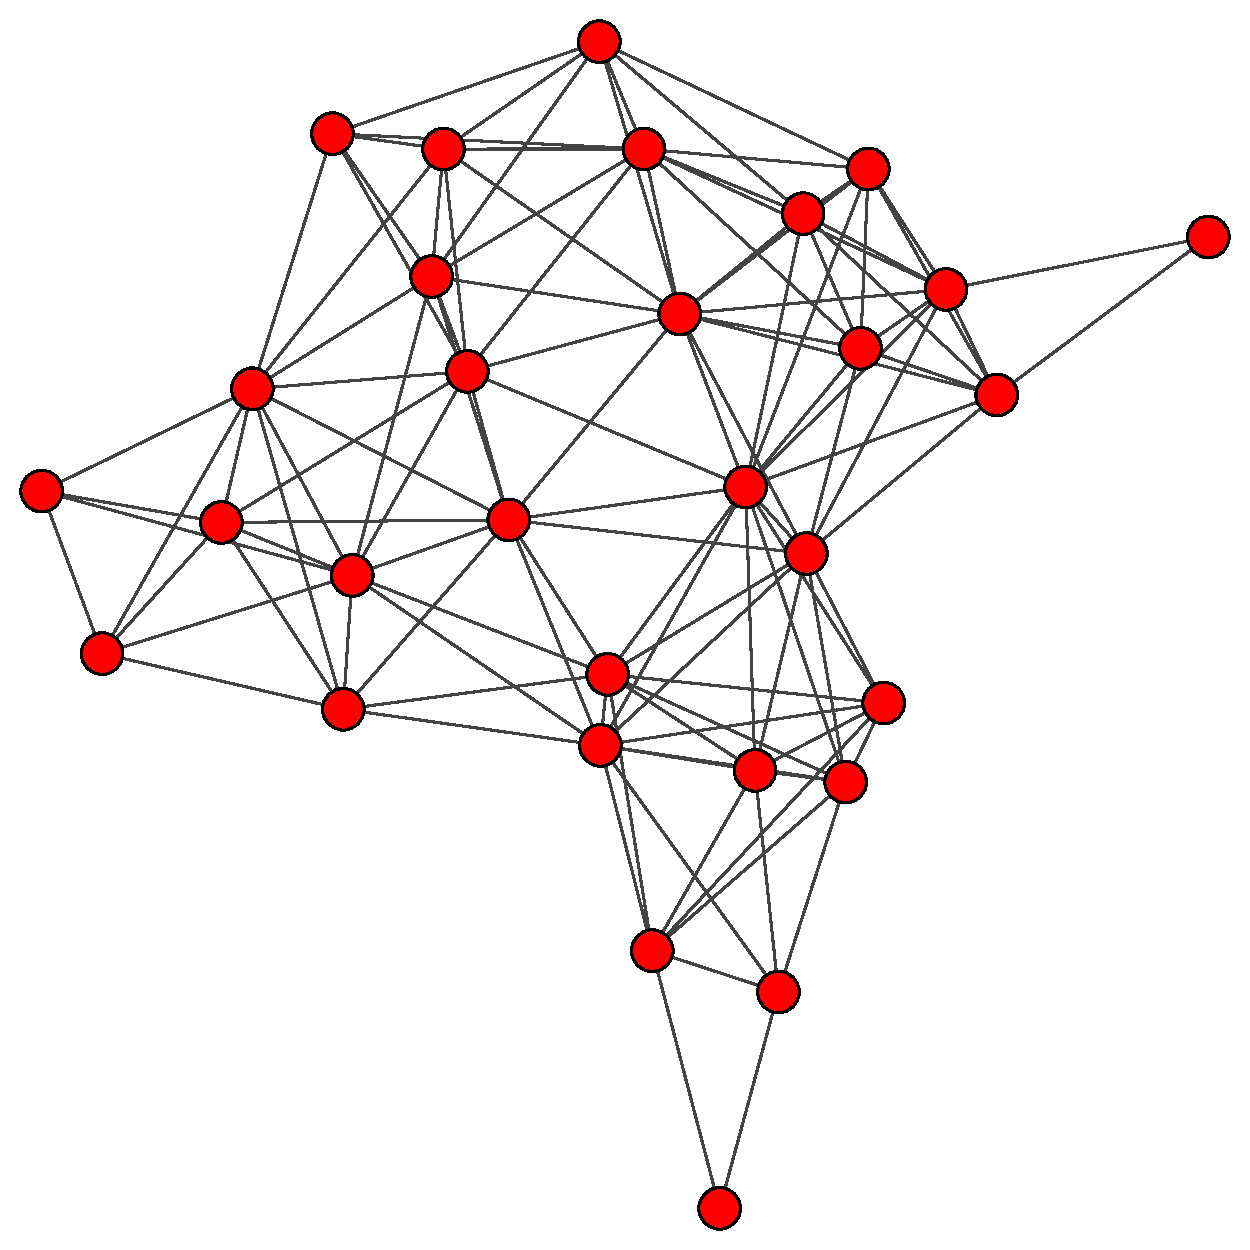
\includegraphics[height=.8\textheight]{fig/mst-0.pdf}
    \end{center}
\end{frame}
\begin{frame}{Exemple 1 : arbre couvrant minimal (non pondéré)}
    \begin{center}
        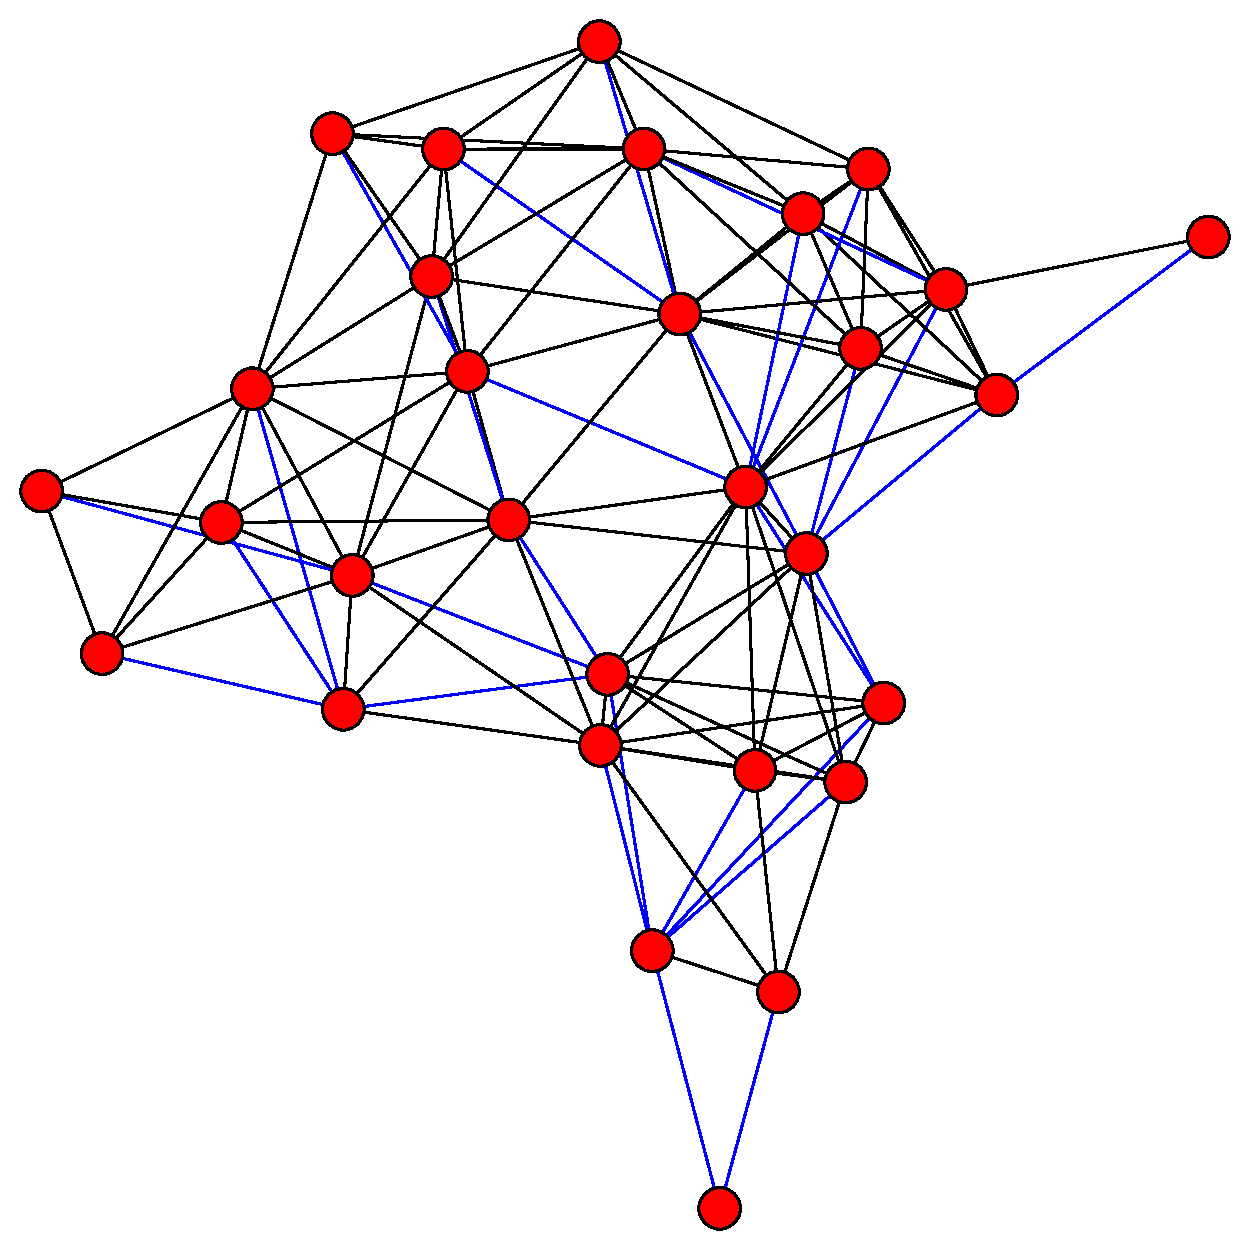
\includegraphics[height=.8\textheight]{fig/mst-1.pdf}
    \end{center}
\end{frame}
\begin{frame}{Exemple 1 : arbre couvrant minimal (non pondéré)}
    \begin{center}
        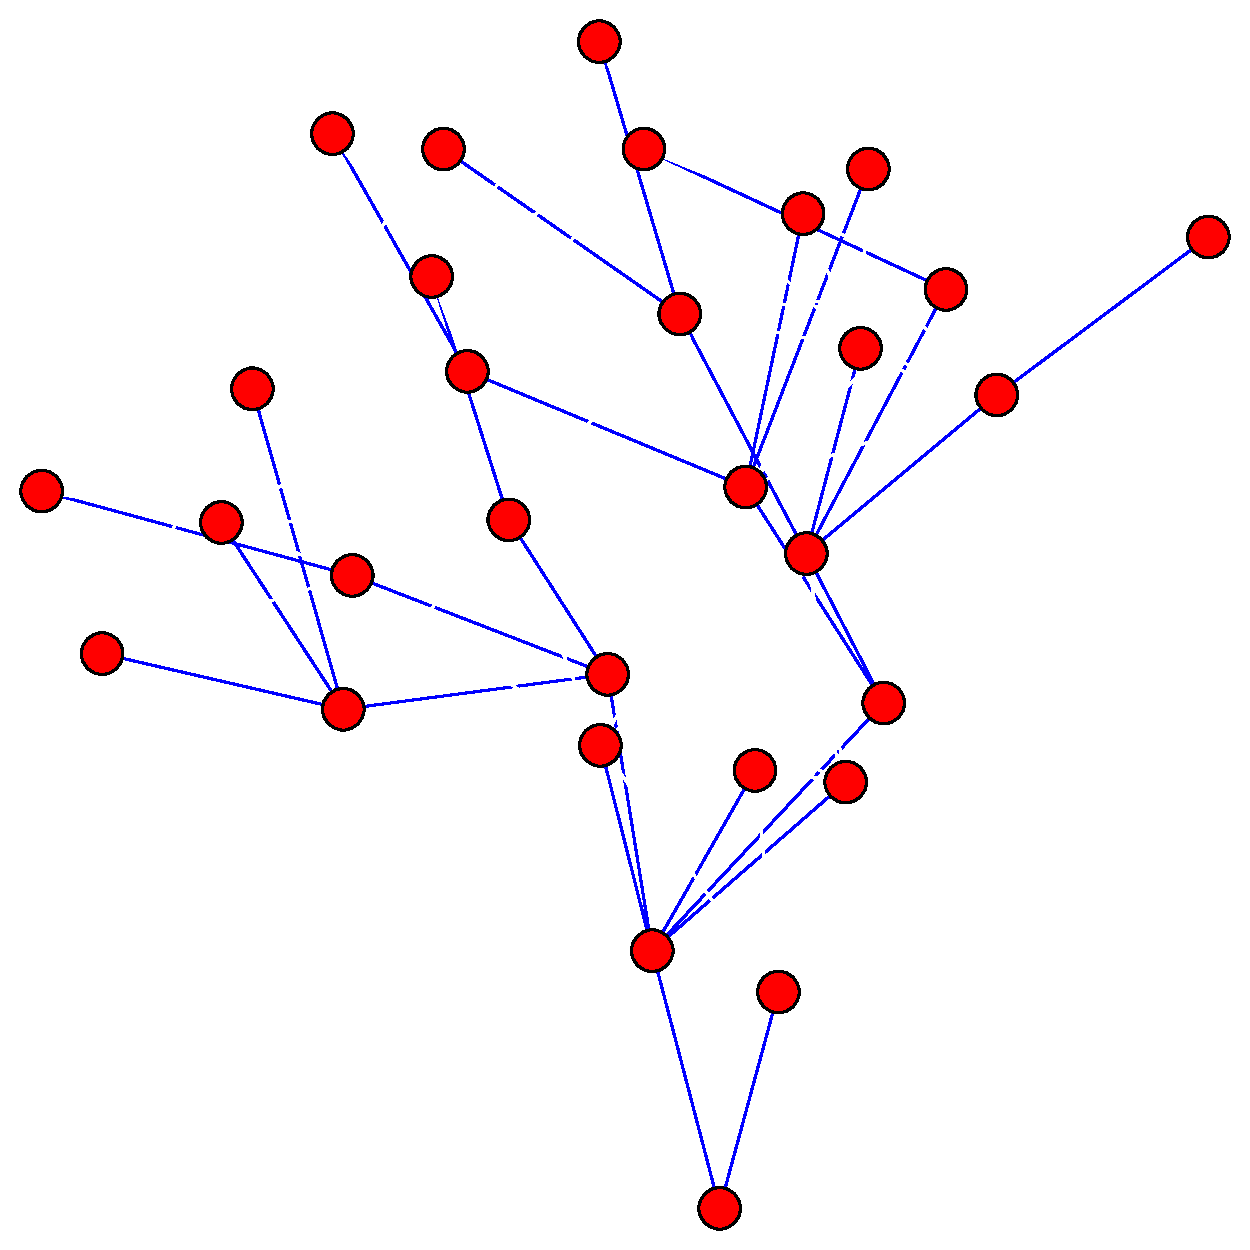
\includegraphics[height=.8\textheight]{fig/mst-2.pdf}
    \end{center}
\end{frame}

\begin{frame}{Exemple 2 : arbre couvrant minimal (pondéré)}
    \begin{center}
        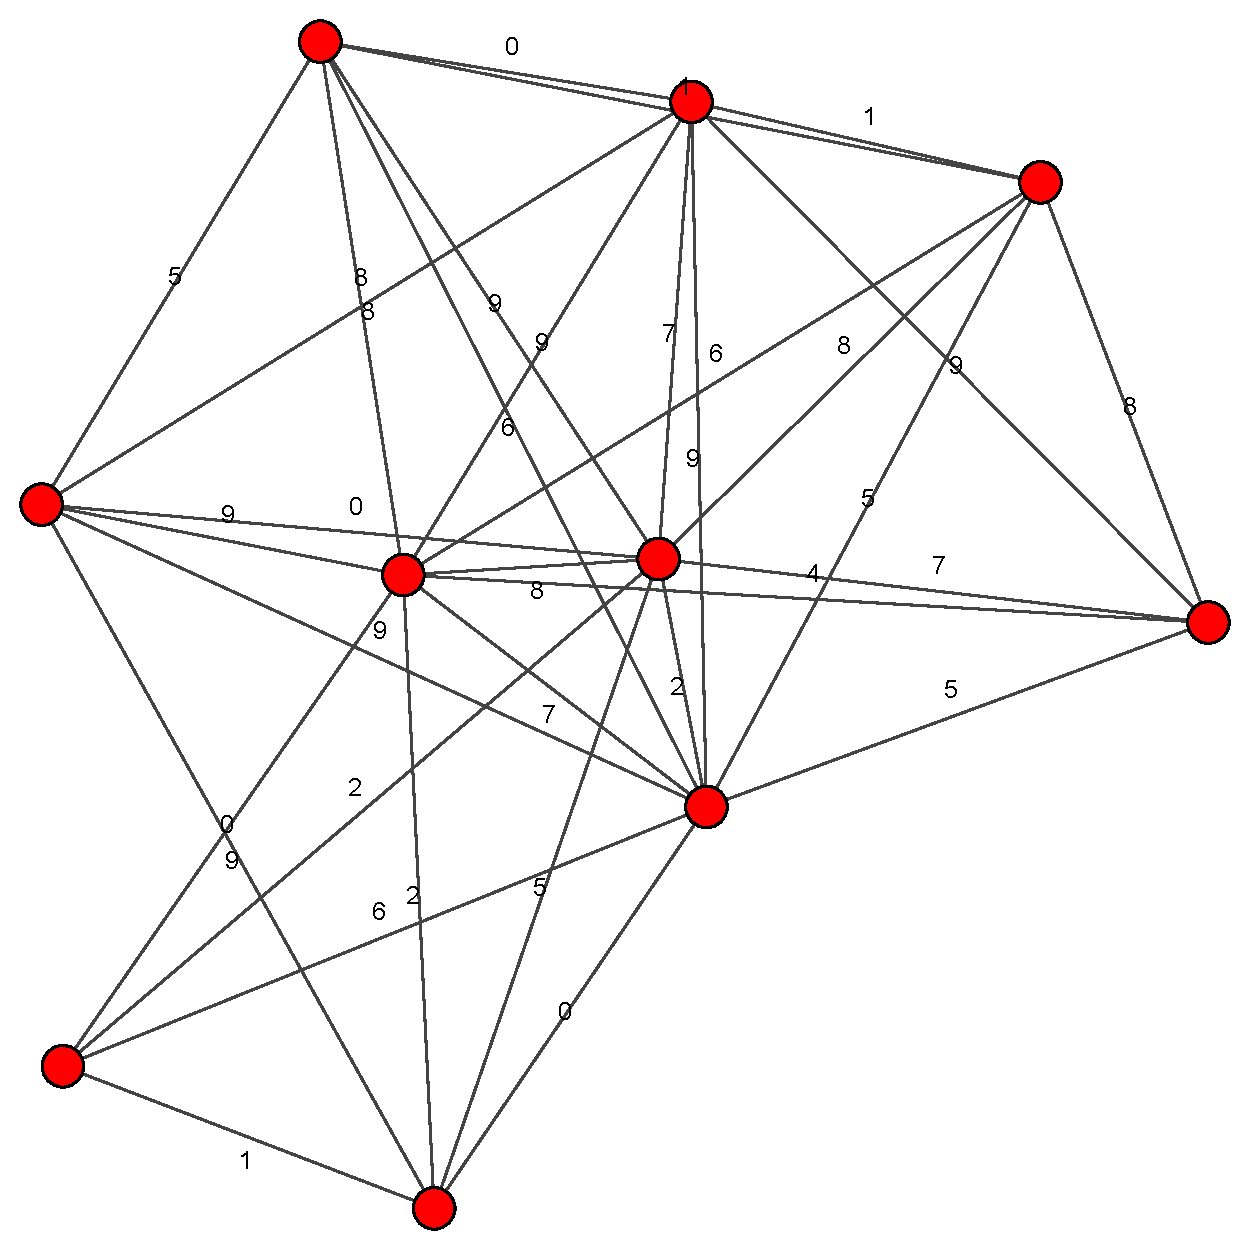
\includegraphics[height=.8\textheight]{fig/mstp-0.pdf}
    \end{center}
\end{frame}
\begin{frame}{Exemple 2 : arbre couvrant minimal (non pondéré)}
    \begin{center}
        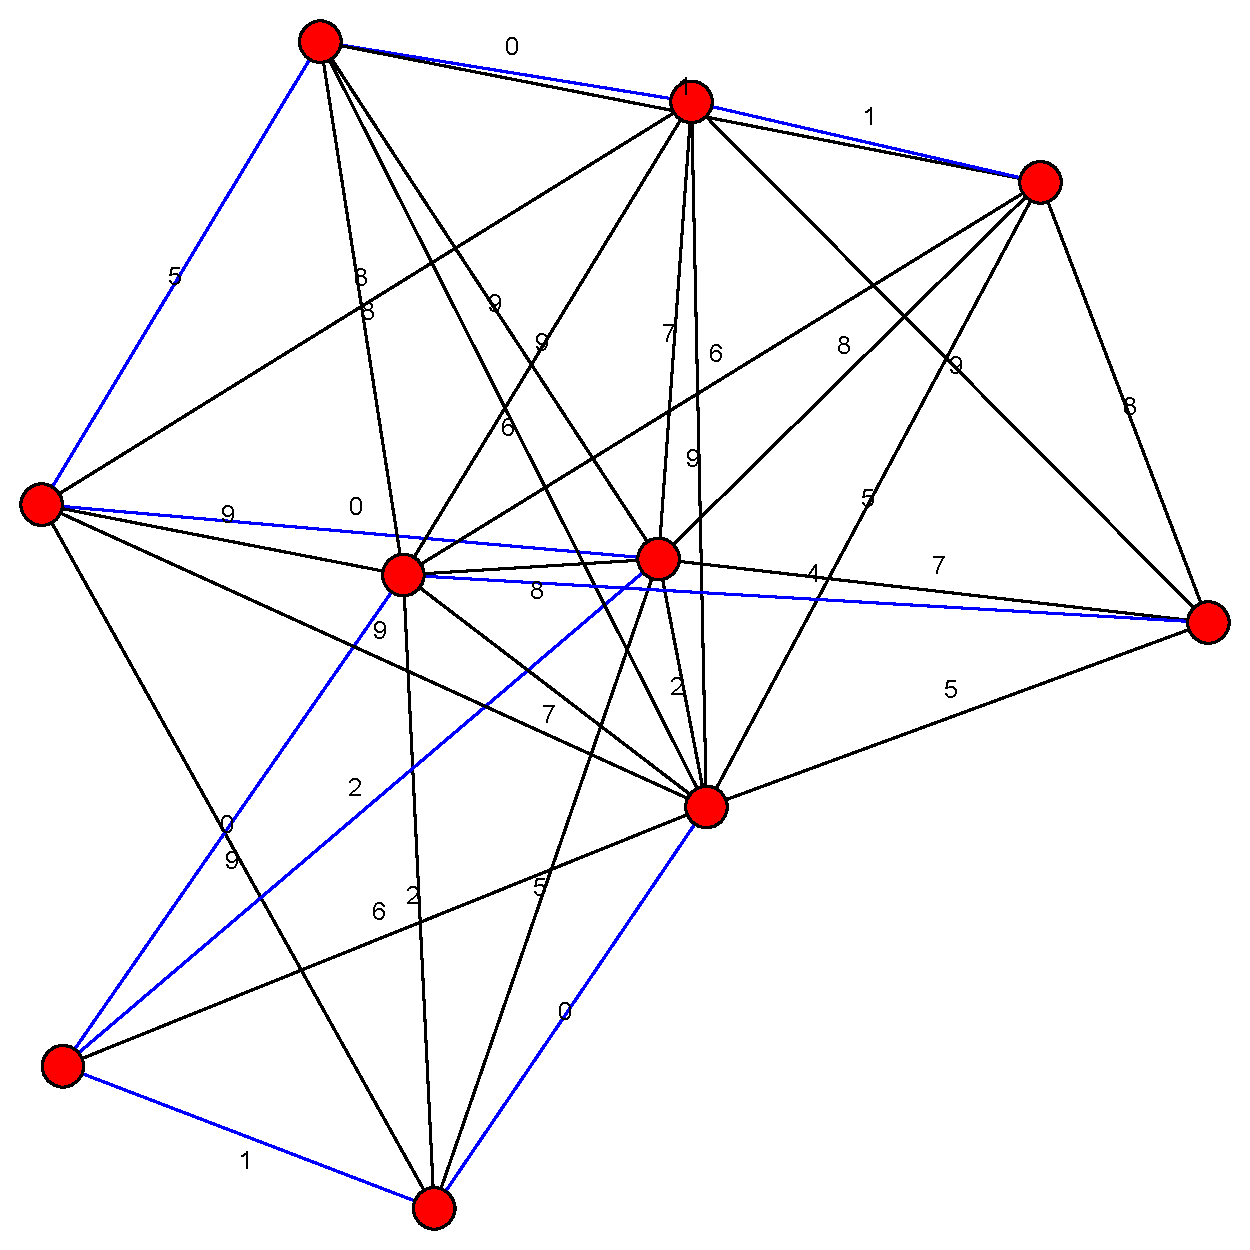
\includegraphics[height=.8\textheight]{fig/mstp-1.pdf}
    \end{center}
\end{frame}

\begin{frame}{Quelques ropriétés}
    \begin{block}{Propriété}
        Ajouter une arête à un graphe non-orienté connexe, crée un cycle
    \end{block}
    L'arête $a$ ajoutée connecte deux sommets $i$ et $j$. Or, le graphe étant connexe, il existait un chemin entre $i$ et $j$ dans le graphe initial. Ajouter $a$ à ce chemin crée un cycle.  
\end{frame}

\begin{frame}{Quelques propriétés}
    \begin{block}{Propriété}
        Enlever une arête à un arbre le rend non-connexe. L'arbre a alors exactement deux composantes connexes. 
    \end{block}
    On note $T-a$ l'arbre privé d'une arête quelconque $a$. On le suppose toujours connexe. Si on ajoute $a$ et qu'on applique la propriété précédente, $T-a$ auquel on a ajouté possède un cycle, ce qui est contradictoire avec le fait que $T$ est un arbre. 
\end{frame}

\begin{frame}{Coupe}
    \begin{definition}
        Une coupe associée à un graphe $G=(S,A)$ est une partition de l'ensemble des sommets $S$ en deux ensembles disjoints $S_1$ et $S_2$. Une arête traversante est une arête $(i,j)$ telle que $i \in S_1$ et $j \in S_2$. 
    \end{definition}
\end{frame}

\begin{frame}{Propriété des cycles}

    \begin{block}{Hypothèse}
        On considère un graphe non-orienté pondéré connexe. On suppose que toutes ses arêtes ont des poids différents
    \end{block}

    Cela assure l'unicité d'un arbre couvrant minimal (admis). Les algorithmes que nous allons voir n'ont pas besoin de cette hypothèse mais l'arbre couvrant minimal n'est plus unique. 
    
    \begin{block}{Propriété}
        Soit $C$ un cycle de $G$. Soit une $f$ une arête de poids maximum dans ce cycle. Alors $f$ n'appartient pas à l'arbre couvrant minimal.
    \end{block}

\end{frame}

\begin{frame}{Démonstration}

    \begin{itemize}
        \item Supposons, par l'absurde que $f$ appartienne à l'arbre couvrant minimal ACM
        \item Enlever $f$ de ACM le coupe en deux composantes connexes 
        \item Il existe une arête $e$ du cycle $C$ qui peut reconnecter les deux composantes 
        \item ACM$-{f}+{e}$ est un nouvel arbre couvrant 
        \item Comme $f$ était l'arête de poids maximum de $C$, ACM$-{f}+{e}$ a un poids inférieur strictement à ACM
        \item Contradiction !
    \end{itemize}
    
\end{frame}

\begin{frame}{Propriété de la coupe}
    
    \begin{block}{Propriété}
        Soit une coupe $S_1,S_2$ de $G$. Soit $e$ l'arête traversante de poids minimum de cette coupe. Alors $e$ appartient forcément à l'arbre couvrant minimal. 
    \end{block}
\end{frame}

\begin{frame}{Démonstration}
    \begin{itemize}
        \item On suppose, par l'absurde, que $e$ n'appartienne pas à l'ACM 
        \item Ajouter $e$ à l'ACM crée alors un cycle 
        \item Il existe une autre arête traversante $f$ qui sépare l'ACM en deux composantes connexes 
        \item ACM$-{f}+{e}$ est nouvel arbre couvrant 
        \item Son poids total est strictement inférieur à celui de ACM 
        \item Contradiction !
    \end{itemize}
\end{frame}

% TODO algorithme glouton 

\begin{frame}{Schéma d'un algorithme glouton}
    \begin{itemize}
        \item On colorie toutes les arêtes de $G$ en noir. On va progressivement colorier en rouge les arêtes de l'arbre couvrant minimal 
        \item On choisit une coupe avec aucune arête traversante rouge 
        \item On sélectionnne l'arête traversante de poids minimum et on la colorie en rouge 
        \item On répète jusqu'à avoir obtenu l'ACM. Combien d'arêtes faut-il ? 
        \begin{itemize}
            \item l'arbre couvrant minimal comporte $n-1$ arêtes 
        \end{itemize}
    \end{itemize}
\end{frame}

\begin{frame}{Correction de l'algorithme}
    \begin{itemize}
        \item Par propriété de la coupe, toutes les arêtes rouges sont dans ACM 
        \item Tant qu'il y a moins de $n-1$ arêtes rouges, on pourra toujours trouver une coupe 
        \begin{itemize}
            \item tant que la forêt noire n'est pas couvrante, ou pas connexe 
        \end{itemize}
    \end{itemize}
\end{frame}

\directlua{\detokenize{
    for i=1,8,1 do
        tex.sprint("\\begin{frame}{Exemple}\\begin{center} \\includegraphics[height=.8\\textheight]{fig/mst-greedy-", i, ".pdf} \\end{center} \\end{frame}")
    end
}}

% TODO algorithme de Prim 

